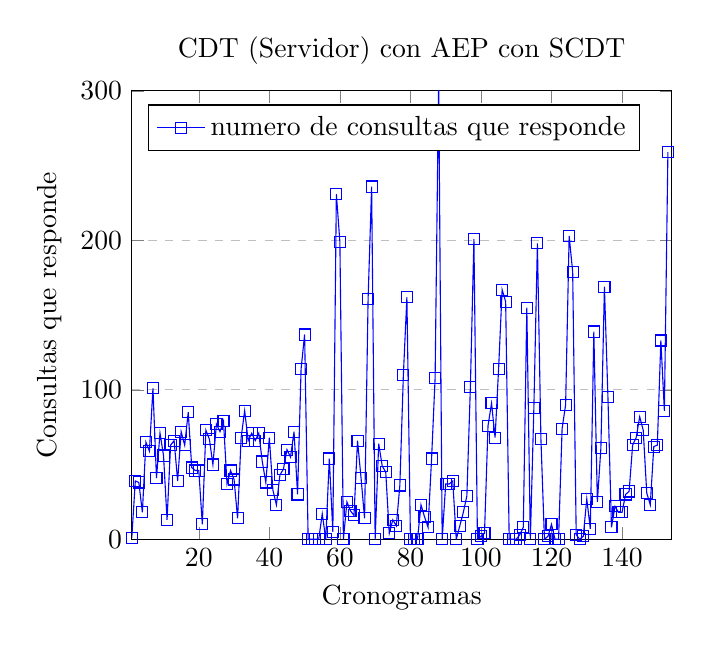
\begin{tikzpicture}
\begin{axis}[
    title={CDT (Servidor) con AEP con SCDT},
    xlabel={Cronogramas},
    ylabel={Consultas que responde},
    xmin=1, xmax=154,
    ymin=0, ymax=300,
    xtick={},
    ytick={},
    legend pos=north west,
    ymajorgrids=true,
    grid style=dashed,
]

\addplot[
    color=blue,
    mark=square,
    ]
    coordinates {
   %CARGA DE TRABAJO Servidor
(1,1)
(2,39)
(3,38)
(4,18)
(5,65)
(6,59)
(7,101)
(8,41)
(9,71)
(10,56)
(11,13)
(12,63)
(13,66)
(14,39)
(15,72)
(16,63)
(17,85)
(18,48)
(19,46)
(20,46)
(21,10)
(22,73)
(23,67)
(24,50)
(25,77)
(26,72)
(27,79)
(28,37)
(29,46)
(30,40)
(31,14)
(32,68)
(33,86)
(34,66)
(35,71)
(36,66)
(37,71)
(38,52)
(39,38)
(40,68)
(41,33)
(42,23)
(43,43)
(44,47)
(45,60)
(46,55)
(47,72)
(48,30)
(49,114)
(50,137)
(51,0)
(52,0)
(53,0)
(54,0)
(55,17)
(56,0)
(57,54)
(58,5)
(59,231)
(60,199)
(61,0)
(62,25)
(63,19)
(64,16)
(65,66)
(66,41)
(67,14)
(68,161)
(69,236)
(70,0)
(71,64)
(72,49)
(73,45)
(74,4)
(75,13)
(76,9)
(77,36)
(78,110)
(79,162)
(80,0)
(81,0)
(82,0)
(83,23)
(84,15)
(85,8)
(86,54)
(87,108)
(88,309)
(89,0)
(90,37)
(91,37)
(92,39)
(93,0)
(94,9)
(95,18)
(96,29)
(97,102)
(98,201)
(99,0)
(100,2)
(101,4)
(102,76)
(103,91)
(104,68)
(105,114)
(106,167)
(107,159)
(108,0)
(109,0)
(110,0)
(111,3)
(112,8)
(113,155)
(114,0)
(115,88)
(116,198)
(117,67)
(118,0)
(119,2)
(120,10)
(121,0)
(122,0)
(123,74)
(124,90)
(125,203)
(126,179)
(127,3)
(128,0)
(129,2)
(130,27)
(131,7)
(132,139)
(133,25)
(134,61)
(135,169)
(136,95)
(137,8)
(138,22)
(139,18)
(140,18)
(141,30)
(142,32)
(143,63)
(144,68)
(145,82)
(146,73)
(147,31)
(148,23)
(149,62)
(150,63)
(151,133)
(152,86)
(153,259)

    };
    \legend{numero de consultas que responde}

\end{axis}
\end{tikzpicture}
